\documentclass[10pt,twocolumn,letterpaper]{article}

\usepackage{cvpr}
\usepackage{times}
\usepackage{epsfig}
\usepackage{graphicx}
\usepackage{amsmath}
\usepackage{amssymb}
\usepackage{verbatim}

% Include other packages here, before hyperref.

% If you comment hyperref and then uncomment it, you should delete
% egpaper.aux before re-running latex.  (Or just hit 'q' on the first latex
% run, let it finish, and you should be clear).
\usepackage[breaklinks=true,bookmarks=false]{hyperref}

\cvprfinalcopy % *** Uncomment this line for the final submission

\def\cvprPaperID{****} % *** Enter the CVPR Paper ID here
\def\httilde{\mbox{\tt\raisebox{-.5ex}{\symbol{126}}}}

% Pages are numbered in submission mode, and unnumbered in camera-ready
%\ifcvprfinal\pagestyle{empty}\fi
\setcounter{page}{1}
\begin{document}

%%%%%%%%% TITLE
\title{Scene Recognition Using Classical and Learning-Based Image Representations}

\author{
Alexis Shiacolas \and
Jingyi Zhong \and
Ngo Heng Yi \and
You Wu \\
University of Southampton \\
School of Electronics and Computer Science \\
Southampton, SO17 1BJ, United Kingdom \\
{\tt\small
as3n23@soton.ac.uk,
jz14g22@soton.ac.uk,
nhy1n25@soton.ac.uk,
yw29g22@soton.ac.uk}
}

\maketitle
%\thispagestyle{empty}




%%%%%%%%% ABSTRACT
\begin{abstract}
This paper presents a systematic evaluation of conventional computer vision methods for scene recognition on a 15-class dataset with 1500 training images. We implement three progressively complex approaches as required by the coursework specification. Run 1 uses a k-nearest neighbor classifier with tiny image features (16$\times$16), achieving 25.67\% validation accuracy with k=1. Run 2 employs a bag-of-visual-words representation with 8$\times$8 pixel patches and logistic regression, reaching 66.53\% accuracy with 800 visual words. For Run 3, we evaluate multiple feature extraction methods including SIFT, GIST, Dense SIFT in Gaussian pyramid, and spatial pyramid pooling approaches. Our experiments show that spatial information is more important than multi-scale information for scene recognition, with PHOW achieving 70.00\% accuracy. The best result of 72.00\% is obtained by combining Gaussian pyramid and spatial pyramid (PHOW-Gaussian) with Chi-Square kernel approximation and linear SVM. We also find that classifier choice significantly affects performance, with GIST features benefiting more from Random Forest (59.33\%) than linear SVM (38.00\%).
\end{abstract}


%%%%%%%BODY TEXT
%%%\begin{comment}
\section{Introduction}

In recent years, deep convolutional neural networks (CNNs) have become the dominant approach for image classification, achieving substantial improvements in accuracy. Despite their success, these models typically require very large training datasets. For example, YOLO was trained on the ImageNet 1000-class dataset, which contains more than one million images, while the Vision Transformer (ViT) was pre-trained using the JFT-300M dataset and later fine-tuned on smaller datasets \cite{redmon2016you, dosovitskiy2020image}.

By comparison, conventional computer vision methods based on feature extraction are still widely used, particularly when only limited training data are available. These approaches extract discriminative features from images, cluster them to form a visual vocabulary, and represent each image using a histogram of visual words \cite{csurka2004visual}.

This paper presents a series of experiments conducted using the scene category dataset provided in COMP3204 Coursework 2, which was originally introduced by Lazebnik \textit{et al.} \cite{lazebnik2006beyond}. Section 2 introduces the dataset and requirements of the coursework. Section 3 describes a k-nearest neighbour (k-NN) classifier using the “tiny image” representation. Section 4 focuses on linear classifiers built upon a bag-of-visual-words model derived from densely sampled fixed-size image patches. Finally, Section 5 compares the performance of different conventional computer vision approaches using k-NN and linear SVM classifiers, and contrasts their results with those obtained using AlexNet trained on the same dataset.

\section{Dataset and Evaluation}

\subsection{Dataset}
We use the scene recognition dataset provided for COMP3204 Coursework 2. The training set consists of 15 scene categories, with 100 images per class, giving us a total of 1500 labelled training images to work with. All images are formatted as JPEG and are greyscale, so colour information is irrelevant for all of the runs.

The test set contains 2985 unlabelled images. In compliance with the restrictions in the coursework brief, these testing images were strictly used to only generate the final predictions for each run and are not used for training, validation, vocabulary learning, or hyperparameter tuning at any stage of development.

\subsection{Evaluation Metric}
We evaluate performance using the coursework objective measure, referred to as average precision. In this context, the average precision corresponds to the classification accuracy, defined as the proportion of correctly classified images out of the total number of predictions on the test data (2985 images).

\subsection{Evaluation Protocol}
All model selection and hyperparameter tuning are carried out exclusively on the training dataset. For each run, relevant hyperparameters are selected by using validation data that is held out from the training set. After tuning, the optimal configuration is retrained on the full training set and used to make final predictions on the test set.

For Run 1, the number of nearest neighbours \textit{k} used by the kNN classifier is selected based on validation performance on the training set.

For Run 2, model performance is evaluated using 5-fold cross-validation on the training set. Hyperparameters such as the visual vocabulary size and classifier regularization are selected based on the mean validation accuracy across folds.

For Run 3, we use a 90\%-10\% split on the training set to create a training subset (1350 images) and a validation subset (150 images). Different feature extraction methods are evaluated, and hyperparameters such as the SVM regularization parameter C and the number of visual words are tuned based on validation accuracy. The random seed is fixed to ensure reproducibility.

\subsection{Output Format}
For each run, the predictions are written to a text file named runX.txt, where X denotes the run number. Each line contains the image filename followed by the predicted scene classifier.

\section{Run 1}
For Run 1, we implement a simple k-nearest neighbours(k-NN) classifier using the "tiny image" representation as a baseline method. Each image is converted to grayscale, center-cropped to a square around the image center, and then resized to 16x16 using bilinear interpolation. The resulting pixels are flattened into a 256-dimensional feature vector. Each feature vector is centred and L2-normalised to unit length, to reduce sensitivity to global illumination and contrast.

Classification is performed using Euclidean distance in the tiny image feature space. For a given test image, the k closest training examples are identified and the predicted class is selected by majority among the neighbour's labels. In cases where multiple classes receive the same number of votes, ties are resolved by selecting the class whose neighbours have the smallest sum of distances.

The optimal value of k is found and selected by using a validation split derived from the training set. For each class, 20 images are assigned to a validation set, and the remaining 80 images are used for training, resulting in 1200 training images and 300 validation images in total. A random seed is used to ensure reproducibility. We evaluate $k \in \{1,3,5,7,9,11,15,21\}$ and measure validation accuracy for each value. The best performance was achieved with $k=1$, with an accuracy of 0.2567, with larger k values producing similar but slightly decreasing results as k grew. Thus $k=1$ is selected for the final model.

The final model is then trained on all 1500 training images and applied to the set of 2985 test images to generate the predictions for Run 1. Class labels are taken directly from the training folder names to ensure the correct output format.


\section{Run 2}
In this part, we trained and classified images using a Bag of Visual Words (BoVW) representation. A visual vocabulary is learned using K-Means clustering, and each image is represented as a histogram of visual word frequencies. Classification is performed using a one-vs-all Logistic Regression approach.

All input images are processed in grayscale to reduce the dimension and complexity of computation, which is consistent with the provided dataset. Images are labelled  and converted into arrays for feature extraction.

In order to build the visual vocabulary, 8 * 8 image patches are extracted by taking 4 pixels in both the x and y directions from the training images. All extracted patches are aggregated and individually mean-centred and L2-normalised. K-Means clustering is then applied to learn a fixed number of visual words forming the vocabulary.

During the classifier training, BoVW histograms have been converted using the learned vocabulary. The feature vectors are then standardised. For each category, a set of binary one-vs-all Logistic Regression classifiers is trained.

The performance of the model is evaluated using a k-fold cross-validation on the training set with k = 5. The number of clusters is 800. For each iteration, the training set was split into a training and validation set with an 8:2 ratio, respectively, while the testing images were excluded entirely from training and tuning. The final reported performance is the mean validation accuracy across folds, which is 0.6653 with a standard deviation of 0.0223. In addition, the number of clusters has been evaluated using values 500, 600, 800, 1000, 1500 and 2000. The result shows that

%------------------------------------------------
\section{Run 3}

For Run 3, we explore different feature extraction methods and classifiers to find the best combination for scene recognition. We evaluate several conventional computer vision approaches including SIFT-based Bag-of-Visual-Words, GIST global descriptors, and spatial pyramid methods. All experiments use a consistent 90\%-10\% train-validation split with a fixed random seed for reproducibility.

\subsection{Feature Extraction Methods}

\subsubsection{SIFT Bag-of-Visual-Words}
We extract standard SIFT descriptors using OpenCV's implementation. Descriptors from all training images are collected and clustered using MiniBatchKMeans with 100 visual words. Each image is then represented as a normalized histogram of visual word frequencies. With 100 visual words, the feature dimension is 100. The max sample parameter limits descriptor sampling to 100,000 for computational efficiency.

\subsubsection{GIST Global Descriptor}
The GIST feature captures global scene properties using Gabor filters at multiple scales and orientations. We use 4 scales, 8 orientations, and a 4$\times$4 spatial grid, resulting in a 512-dimensional feature vector (4$\times$8$\times$16=512). Images are resized to 256$\times$256 before feature extraction. Each Gabor-filtered response is divided into blocks and averaged to form the final descriptor.

\subsubsection{Dense SIFT in Gaussian Pyramid}
This method extracts dense SIFT features at multiple scales of a Gaussian pyramid. We use 3 pyramid scales with a scale factor of 0.7 (original, 0.7$\times$, and 0.49$\times$). Dense SIFT is computed on a grid with 8-pixel spacing. Features from all scales are quantized using 250 visual words, then concatenated to form a 750-dimensional feature (3 scales $\times$ 250 words).

\subsubsection{PHOW (Pyramid Histogram of Words)}
PHOW extends the bag-of-words representation by incorporating spatial pyramid pooling. We use spatial levels [0, 1, 2], which divide the image into grids of 1$\times$1, 2$\times$2, and 4$\times$4 cells, respectively. Dense SIFT descriptors are extracted with 8-pixel spacing and quantized using 250 visual words. The total feature dimension is 5250 (21 cells $\times$ 250 words), with each spatial level weighted by $1/2^L$ where $L$ is the level index.

\subsubsection{PHOW-Gaussian Pyramid}
This method combines both Gaussian pyramid and spatial pyramid approaches. We use 2 Gaussian scales (original and 0.7$\times$) with 2 spatial levels [0, 1] at each scale. This results in 2500 dimensions (2 Gaussian scales $\times$ 5 spatial cells $\times$ 250 words), offering a balance between the multi-scale information of Gaussian pyramids and the spatial layout information of PHOW.

\begin{figure}[t]
\centering
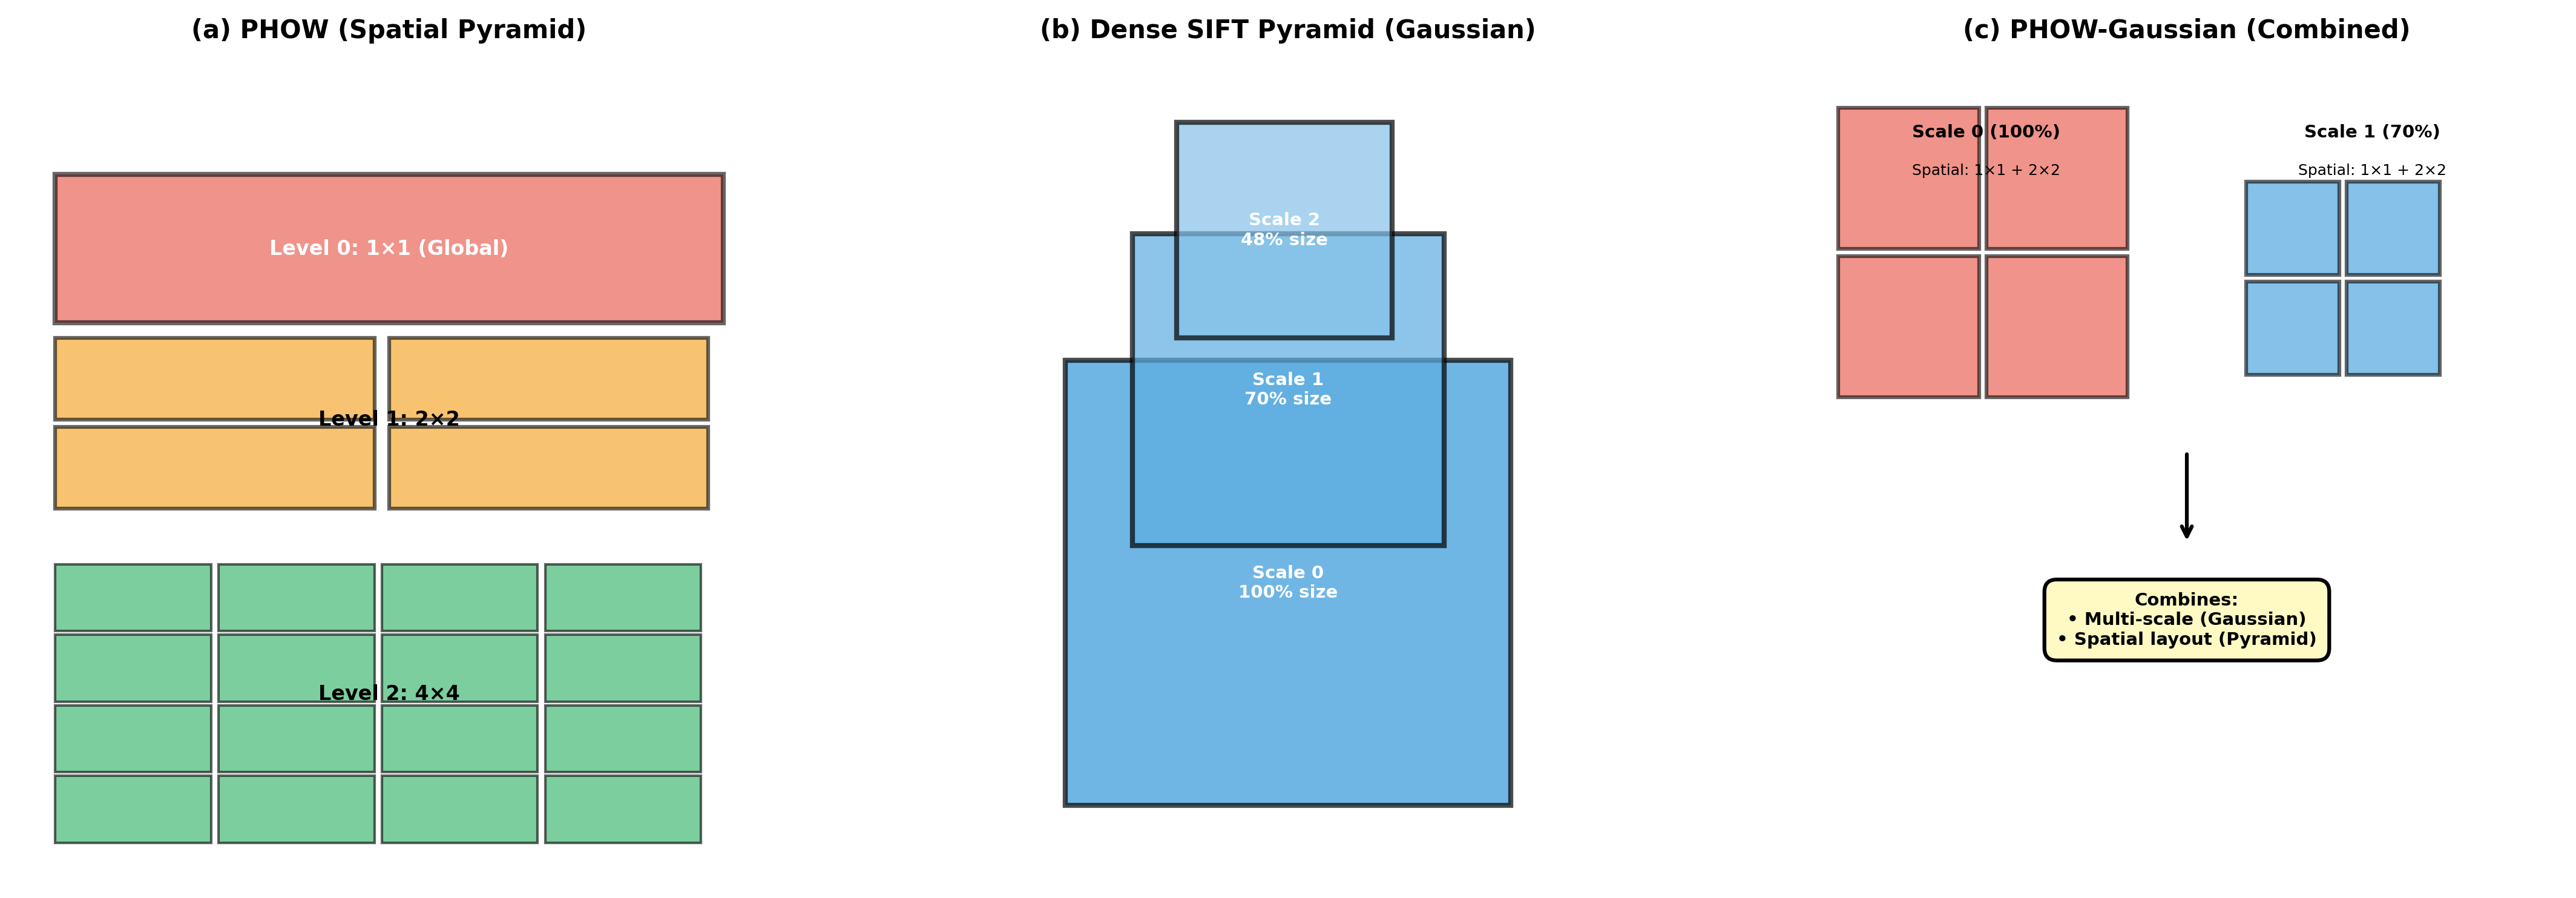
\includegraphics[width=\linewidth]{figures/fig6_architecture_diagram.png}
\caption{Architectural comparison of pyramid-based feature extraction methods. (a) PHOW uses spatial pyramid pooling with three levels (1$\times$1, 2$\times$2, 4$\times$4) to capture spatial layout information. (b) Dense SIFT Pyramid applies Gaussian pyramid to extract features at multiple scales. (c) PHOW-Gaussian combines both approaches, applying spatial pooling at each Gaussian scale to capture both multi-scale and spatial information.}
\label{fig:architecture}
\end{figure}

To provide an intuitive understanding of these pyramid-based approaches, Figure~\ref{fig:architecture} illustrates the architectural differences between the three pyramid methods. PHOW (a) divides the image into increasingly fine spatial grids to capture spatial layout, while Dense SIFT Pyramid (b) processes the image at multiple scales to capture objects of different sizes. PHOW-Gaussian (c) combines these two strategies, applying spatial pooling at each scale level. This architectural visualization helps explain why PHOW-Gaussian achieves better performance by incorporating both types of information.

\subsection{Classification Methods}

\subsubsection{k-Nearest Neighbors}
For SIFT BoVW features, we evaluate k-NN with various k values ranging from 10 to 100. The best validation accuracy is 44.00\% at k=30. The k-NN classifier is simple but performs poorly with high-dimensional features.

\subsubsection{Chi-Square Kernel with Linear SVM}
Since BoVW histograms benefit from non-linear kernels, we use the Chi-Square kernel approximation (AdditiveChi2Sampler) followed by a Linear SVM. For SIFT BoVW features with sample\_steps=3 and C=0.01, we achieve 48.67\% accuracy. This improves over k-NN by approximately 4\%.

\subsubsection{Linear SVM}
We use Linear SVM with L2 regularization for all spatial pyramid features. The regularization parameter C is tuned on the validation set. Different feature types require different C values: GIST performs best at C=10 (38.00\%), while PHOW and PHOW-Gaussian work best at C=0.1.

\subsubsection{Random Forest}
For GIST features, we also evaluate Random Forest classifiers. With 200 trees, the accuracy reaches 59.33\%, which is substantially better than Linear SVM (38.00\%) on the same features. This suggests that GIST features benefit from non-linear classification.

\subsection{Hyperparameter Tuning}

For each method, we tune hyperparameters using validation accuracy. To illustrate the tuning process and the sensitivity of different methods to hyperparameter choices, we present detailed tuning curves for three representative methods in Figure~\ref{fig:hyperparameter_tuning}. We select GIST with Linear SVM, Dense SIFT Pyramid, and PHOW for this analysis because they represent three distinct types of features: global descriptors (GIST), multi-scale local features (Dense SIFT Pyramid), and spatial pyramid features (PHOW). These three methods exhibit different behaviors with respect to the regularization parameter C, making them suitable for demonstrating the importance of proper hyperparameter selection.

\begin{figure}[t]
\centering
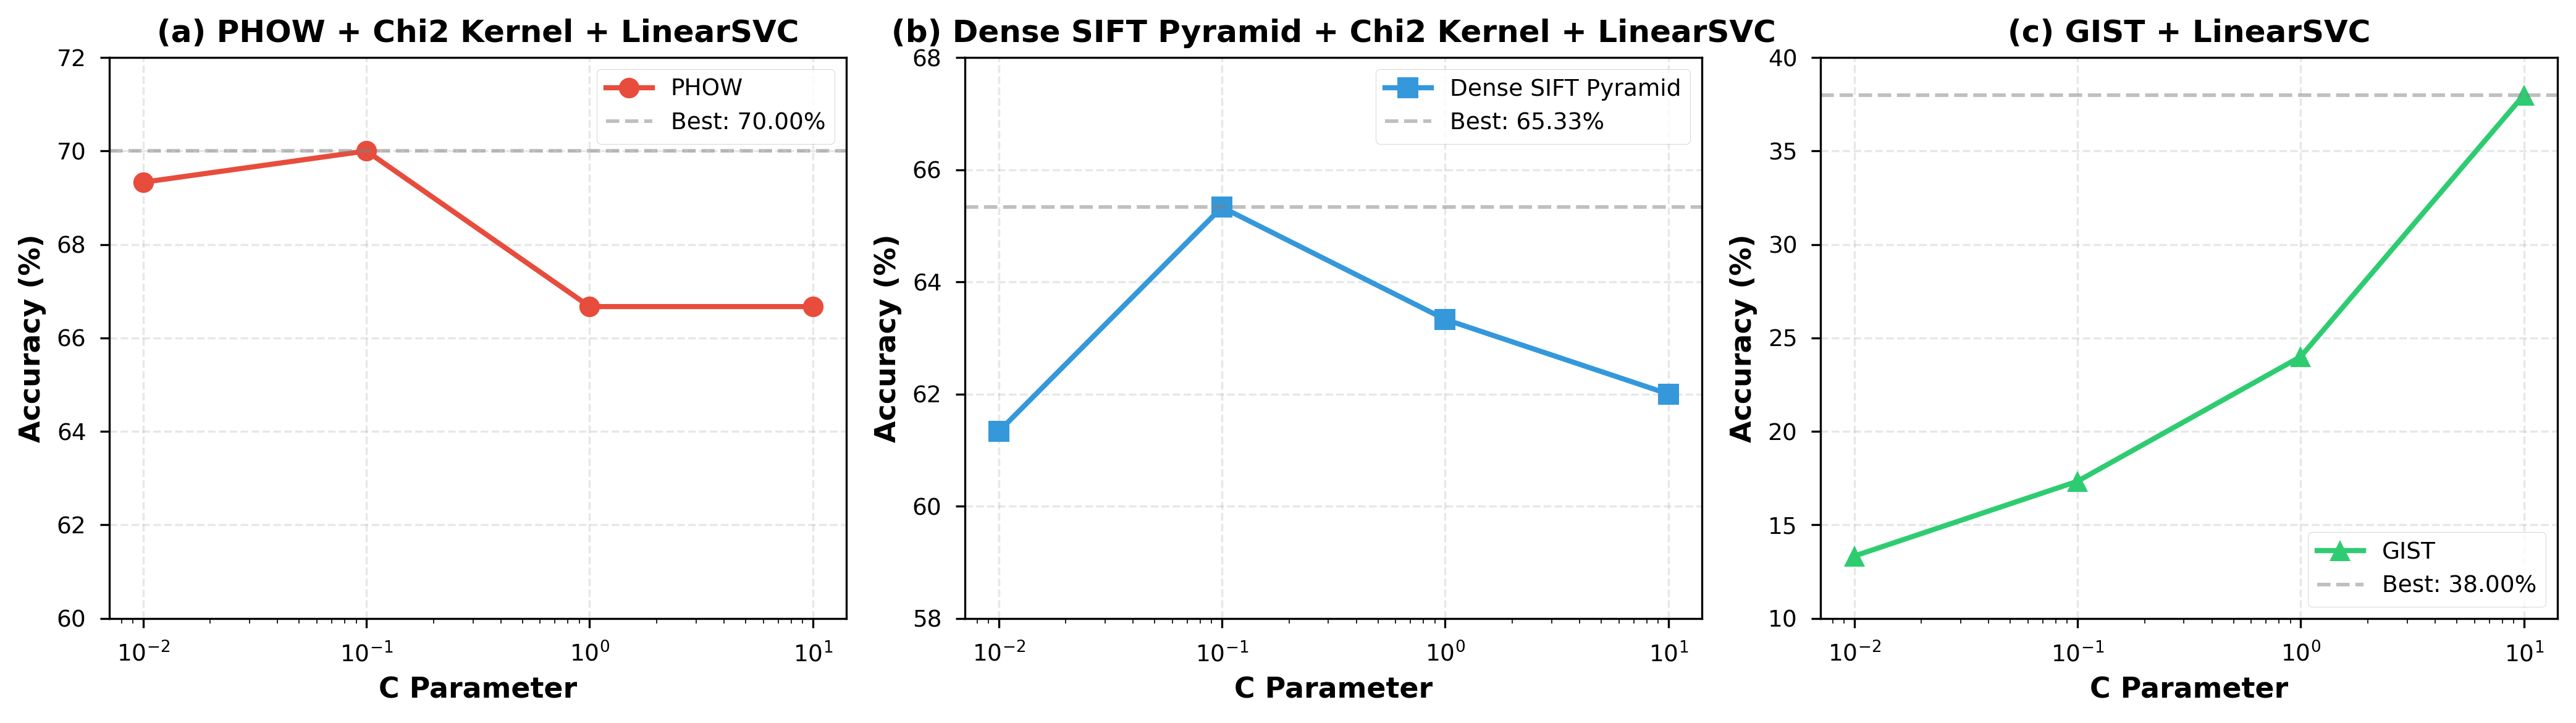
\includegraphics[width=\linewidth]{figures/fig2_hyperparameter_tuning.png}
\caption{Effect of SVM regularization parameter C on validation accuracy for three representative feature methods. Each method shows distinct sensitivity to regularization: GIST requires larger C values (less regularization) and peaks at C=10 with 38.00\% accuracy, while both Dense SIFT Pyramid and PHOW prefer stronger regularization with optimal C=0.1, achieving 65.33\% and 70.00\% respectively. The consistent behavior of pyramid-based methods (Dense SIFT and PHOW) suggests that spatial and multi-scale features benefit from similar regularization strategies.}
\label{fig:hyperparameter_tuning}
\end{figure}

As shown in Figure~\ref{fig:hyperparameter_tuning}, PHOW achieves its optimal performance at C=0.1 with 70.00\% accuracy, while smaller values (C=0.01) and larger values (C=1, 10) result in slightly lower accuracy. Dense SIFT Pyramid exhibits similar behavior, also peaking at C=0.1 with 65.33\% accuracy. In contrast, GIST with Linear SVM shows consistent improvement as C increases, reaching 38.00\% at C=10. This indicates that GIST features require less regularization compared to histogram-based representations. The similar tuning behavior of Dense SIFT Pyramid and PHOW suggests that both spatial pyramid and Gaussian pyramid features benefit from stronger regularization, likely due to their higher dimensionality and histogram-based nature.

\subsection{Results and Analysis}

We evaluate eight different combinations of feature extraction methods and classifiers on the validation set. Figure~\ref{fig:feature_comparison} presents a comprehensive comparison of all methods from two perspectives: overall accuracy ranking and the trade-off between feature dimensionality and classification performance.

\begin{figure}[t]
\centering
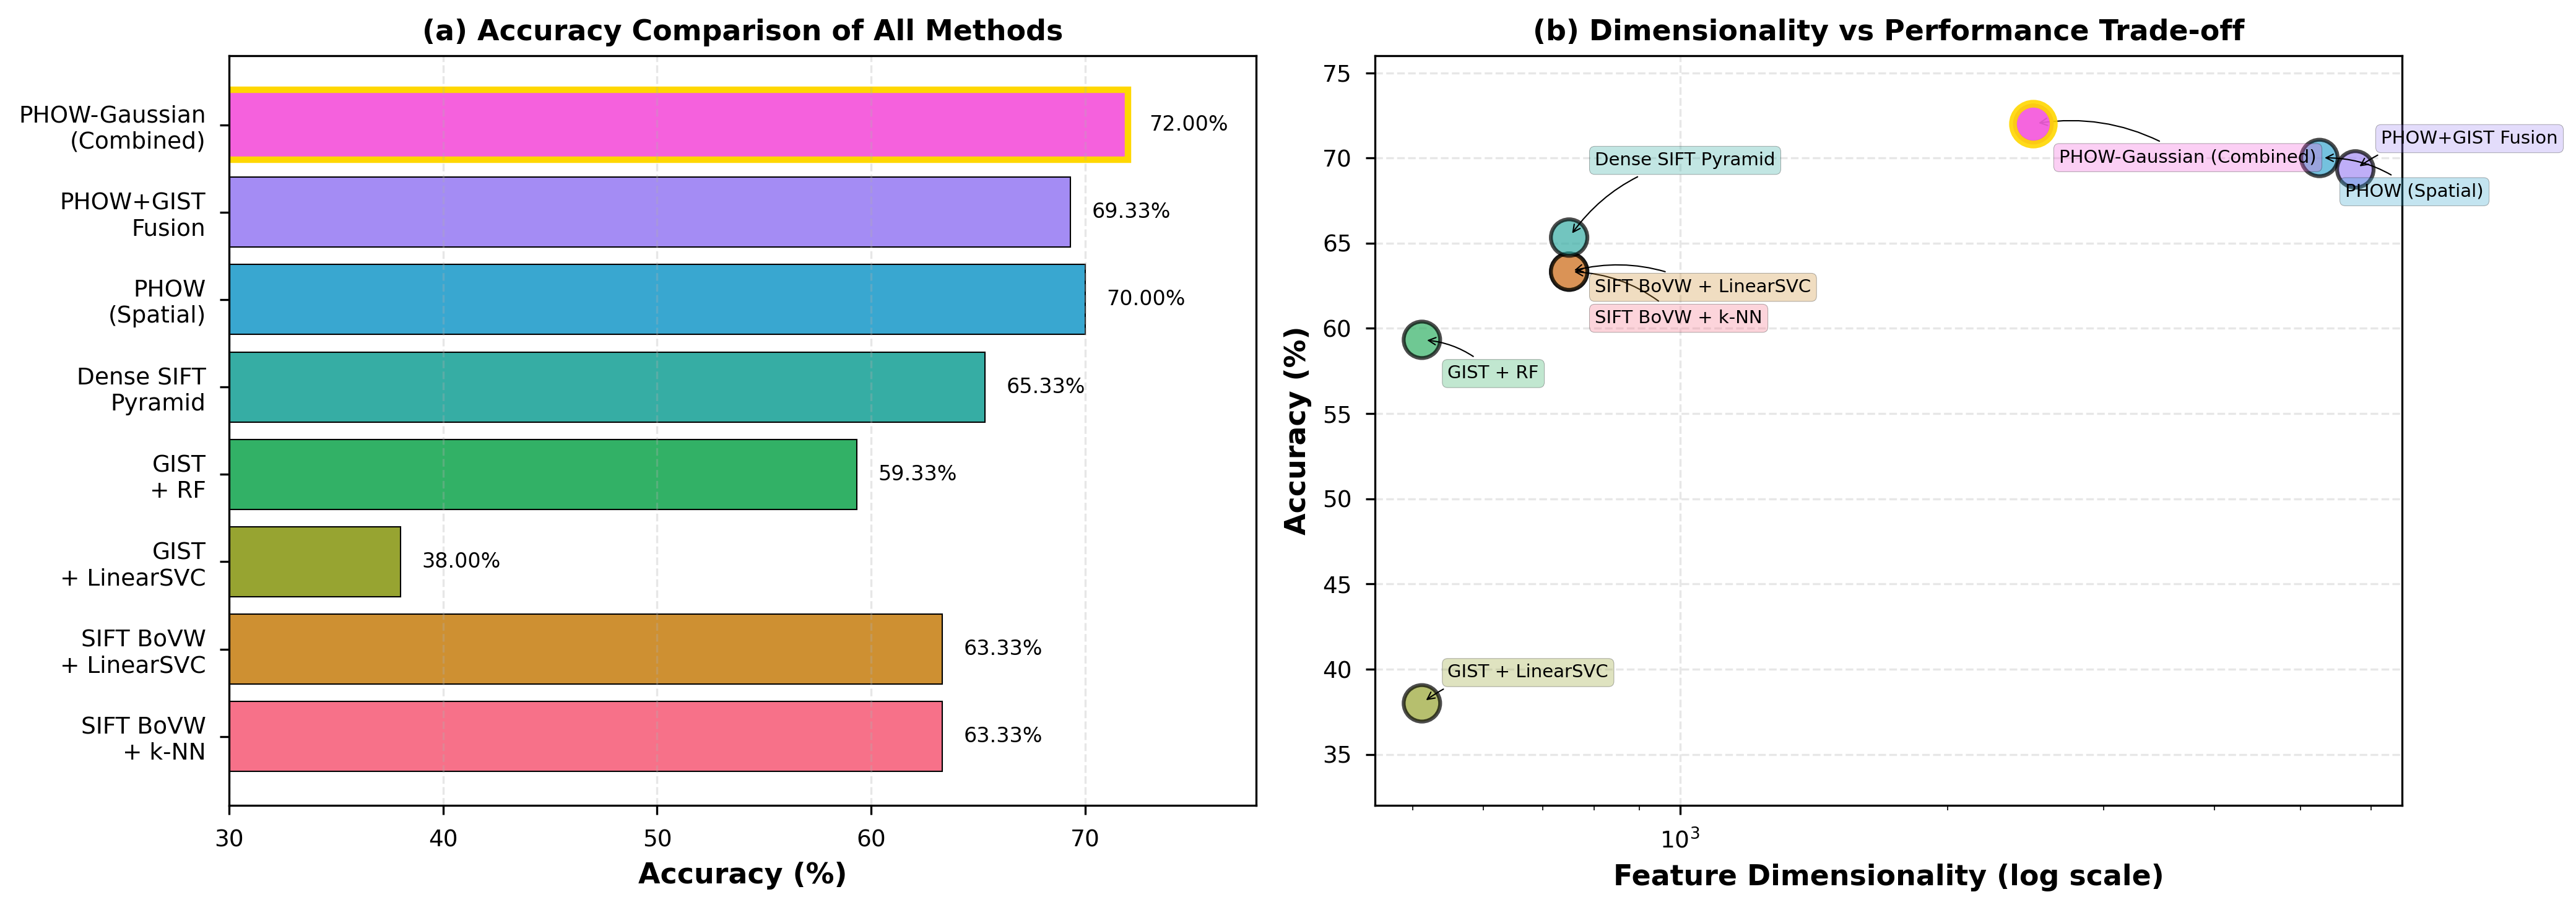
\includegraphics[width=\linewidth]{figures/fig1_feature_comparison.png}
\caption{Comprehensive comparison of all feature extraction methods. (a) Accuracy ranking shows PHOW-Gaussian achieves the highest validation accuracy of 72.00\%, followed by PHOW (70.00\%) and PHOW+GIST fusion (69.33\%). (b) Dimensionality vs performance trade-off reveals that higher dimensionality does not guarantee better performance. PHOW-Gaussian achieves optimal performance with 2500 dimensions, while PHOW uses 5250 dimensions but achieves 2\% lower accuracy. GIST uses only 512 dimensions but shows the largest performance variance depending on classifier choice.}
\label{fig:feature_comparison}
\end{figure}

As shown in Figure~\ref{fig:feature_comparison}(a), PHOW-Gaussian Pyramid achieves the best validation accuracy of 72.00\%, followed by PHOW (70.00\%) and PHOW+GIST fusion (69.33\%). Dense SIFT Pyramid reaches 65.33\%, while basic SIFT BoVW methods achieve 48.67\% with Chi2-LinearSVC and 44.00\% with k-NN. GIST features show the largest performance variance: only 38.00\% with Linear SVM but 59.33\% with Random Forest, indicating that classifier choice is critical for global descriptors.

Figure~\ref{fig:feature_comparison}(b) examines the relationship between feature dimensionality and performance. Notably, higher dimensionality does not guarantee better accuracy. PHOW uses 5250 dimensions but achieves 70.00\%, while PHOW-Gaussian uses only 2500 dimensions yet achieves 72.00\%. This suggests that the combination of multi-scale and spatial information is more important than raw feature dimensionality. GIST features occupy the low-dimensionality region (512 dimensions) with moderate performance, while PHOW+GIST fusion (5762 dimensions) performs slightly worse than PHOW alone, indicating that simply concatenating features does not always improve results.

\begin{figure}[t]
\centering
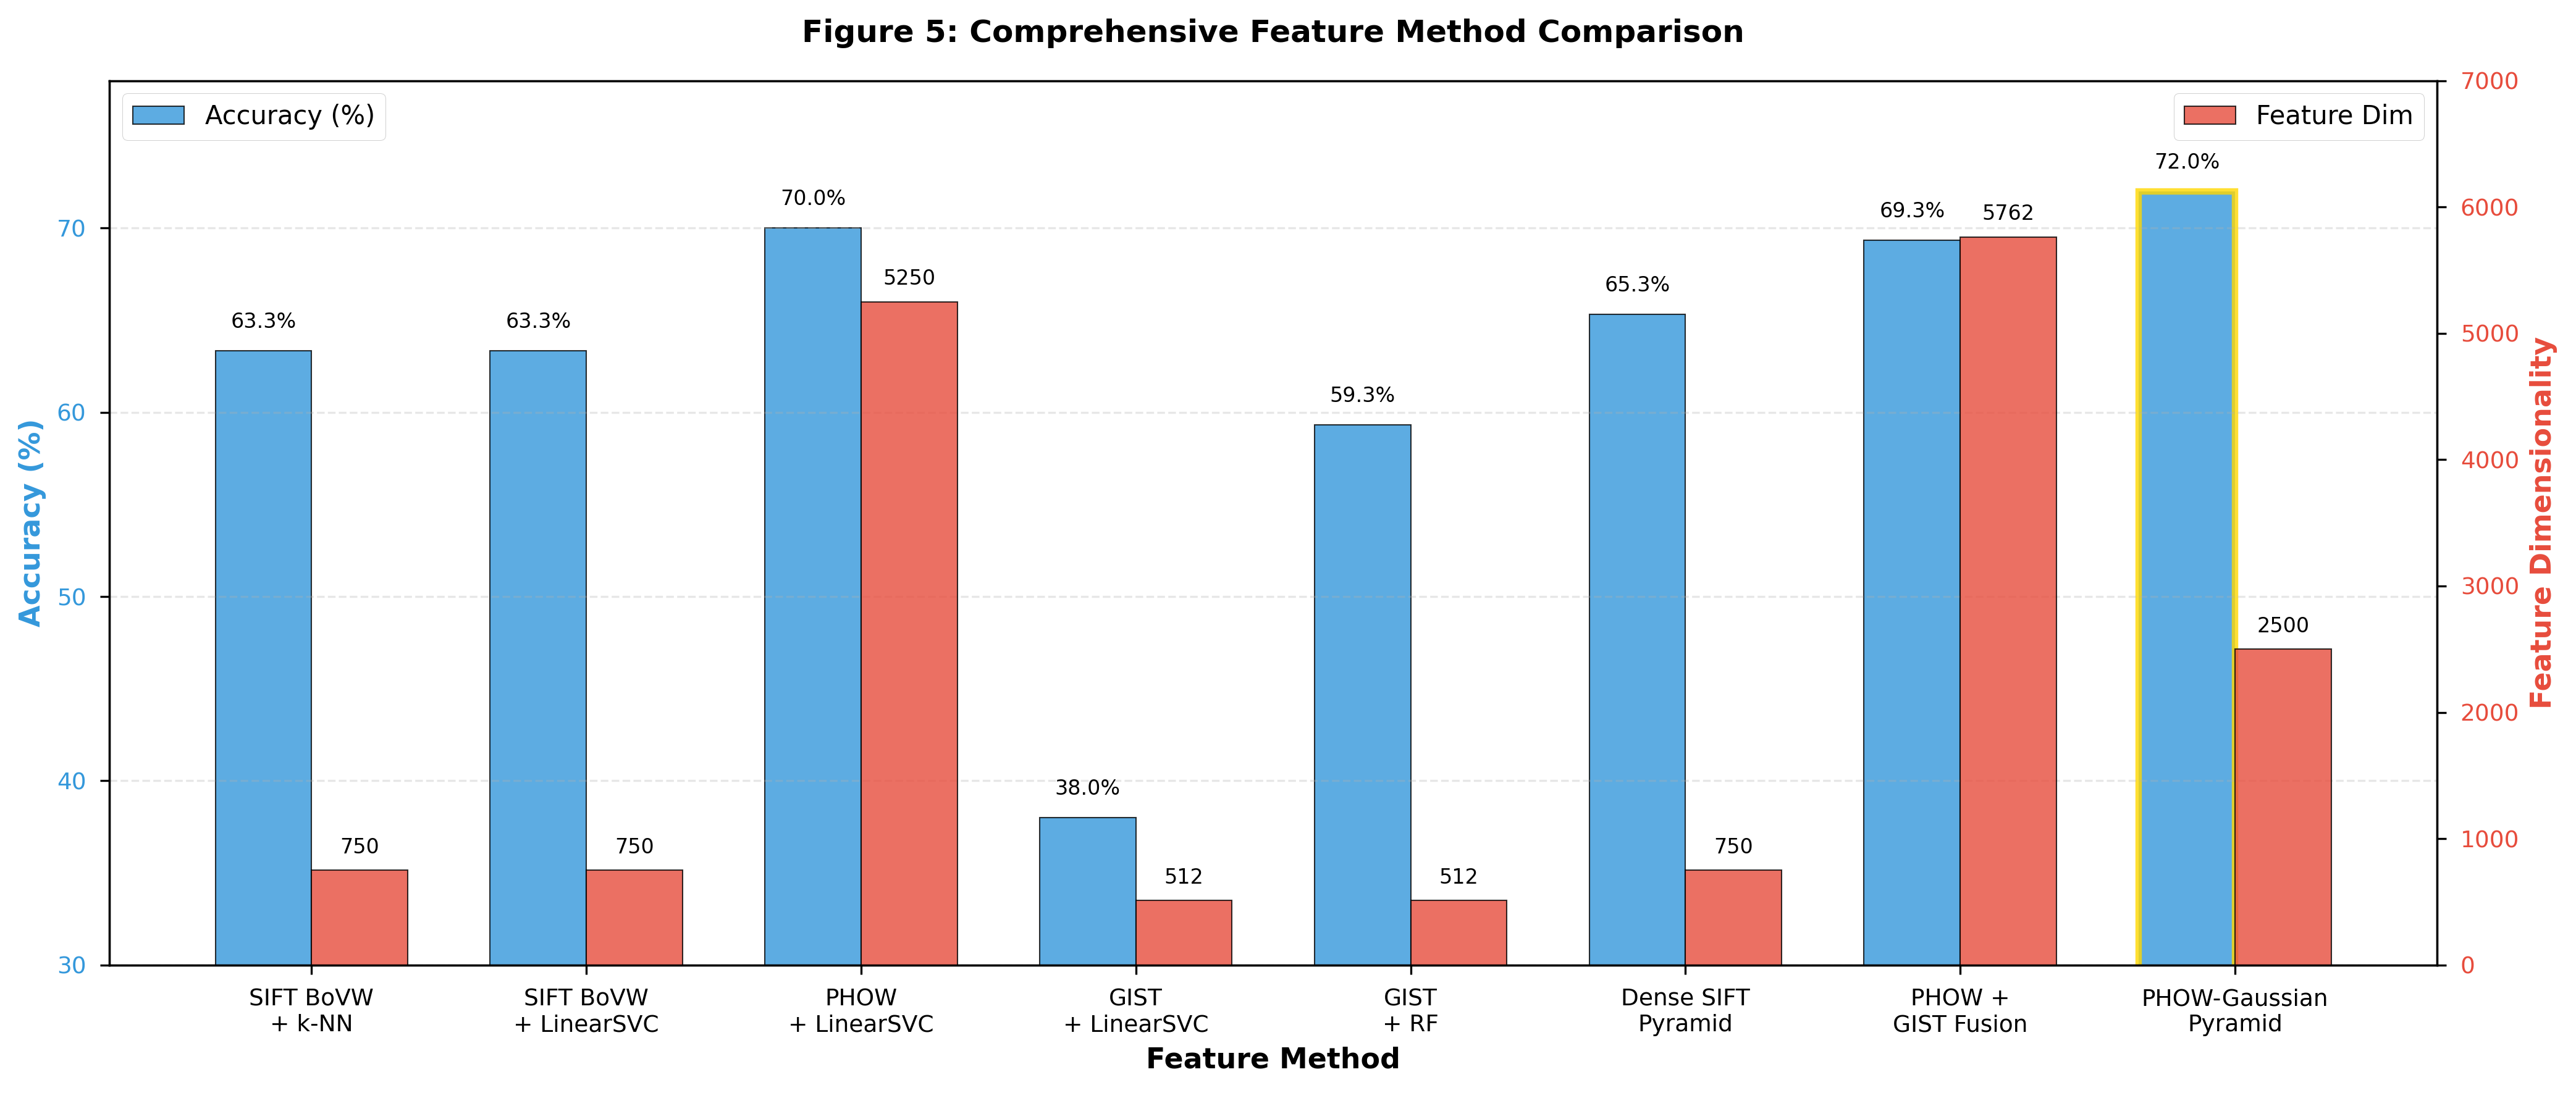
\includegraphics[width=\linewidth]{figures/fig5_feature_fusion.png}
\caption{Detailed comparison of all evaluated methods showing accuracy and feature dimensionality. This dual-axis visualization reveals that feature dimensionality and classification accuracy do not correlate linearly. PHOW-Gaussian achieves the best performance (72.00\%) with moderate dimensionality (2500), while PHOW+GIST fusion uses the highest dimensionality (5762) but achieves lower accuracy (69.33\%). The stark difference between GIST+LinearSVC (38.00\%) and GIST+RF (59.33\%) demonstrates that feature-classifier compatibility is crucial for optimal performance.}
\label{fig:feature_fusion}
\end{figure}

Figure~\ref{fig:feature_fusion} provides a detailed comparison of accuracy and feature dimensionality across all methods. The dual-axis bar chart clearly illustrates that feature dimensionality alone does not determine performance. For instance, both basic SIFT BoVW methods use 100-dimensional features but achieve only 44.00\% (k-NN) and 48.67\% (Chi2-LinearSVC), while Dense SIFT Pyramid with 750 dimensions reaches 65.33\%. This 16-21 percentage point improvement demonstrates the significant benefit of multi-scale feature extraction over simple bag-of-words representations, even when using the same underlying SIFT descriptors. The most striking observation is the performance gap between GIST+LinearSVC (38.00\%) and GIST+RF (59.33\%), which underscores the importance of selecting appropriate classifiers for different feature representations.

\begin{figure}[t]
\centering
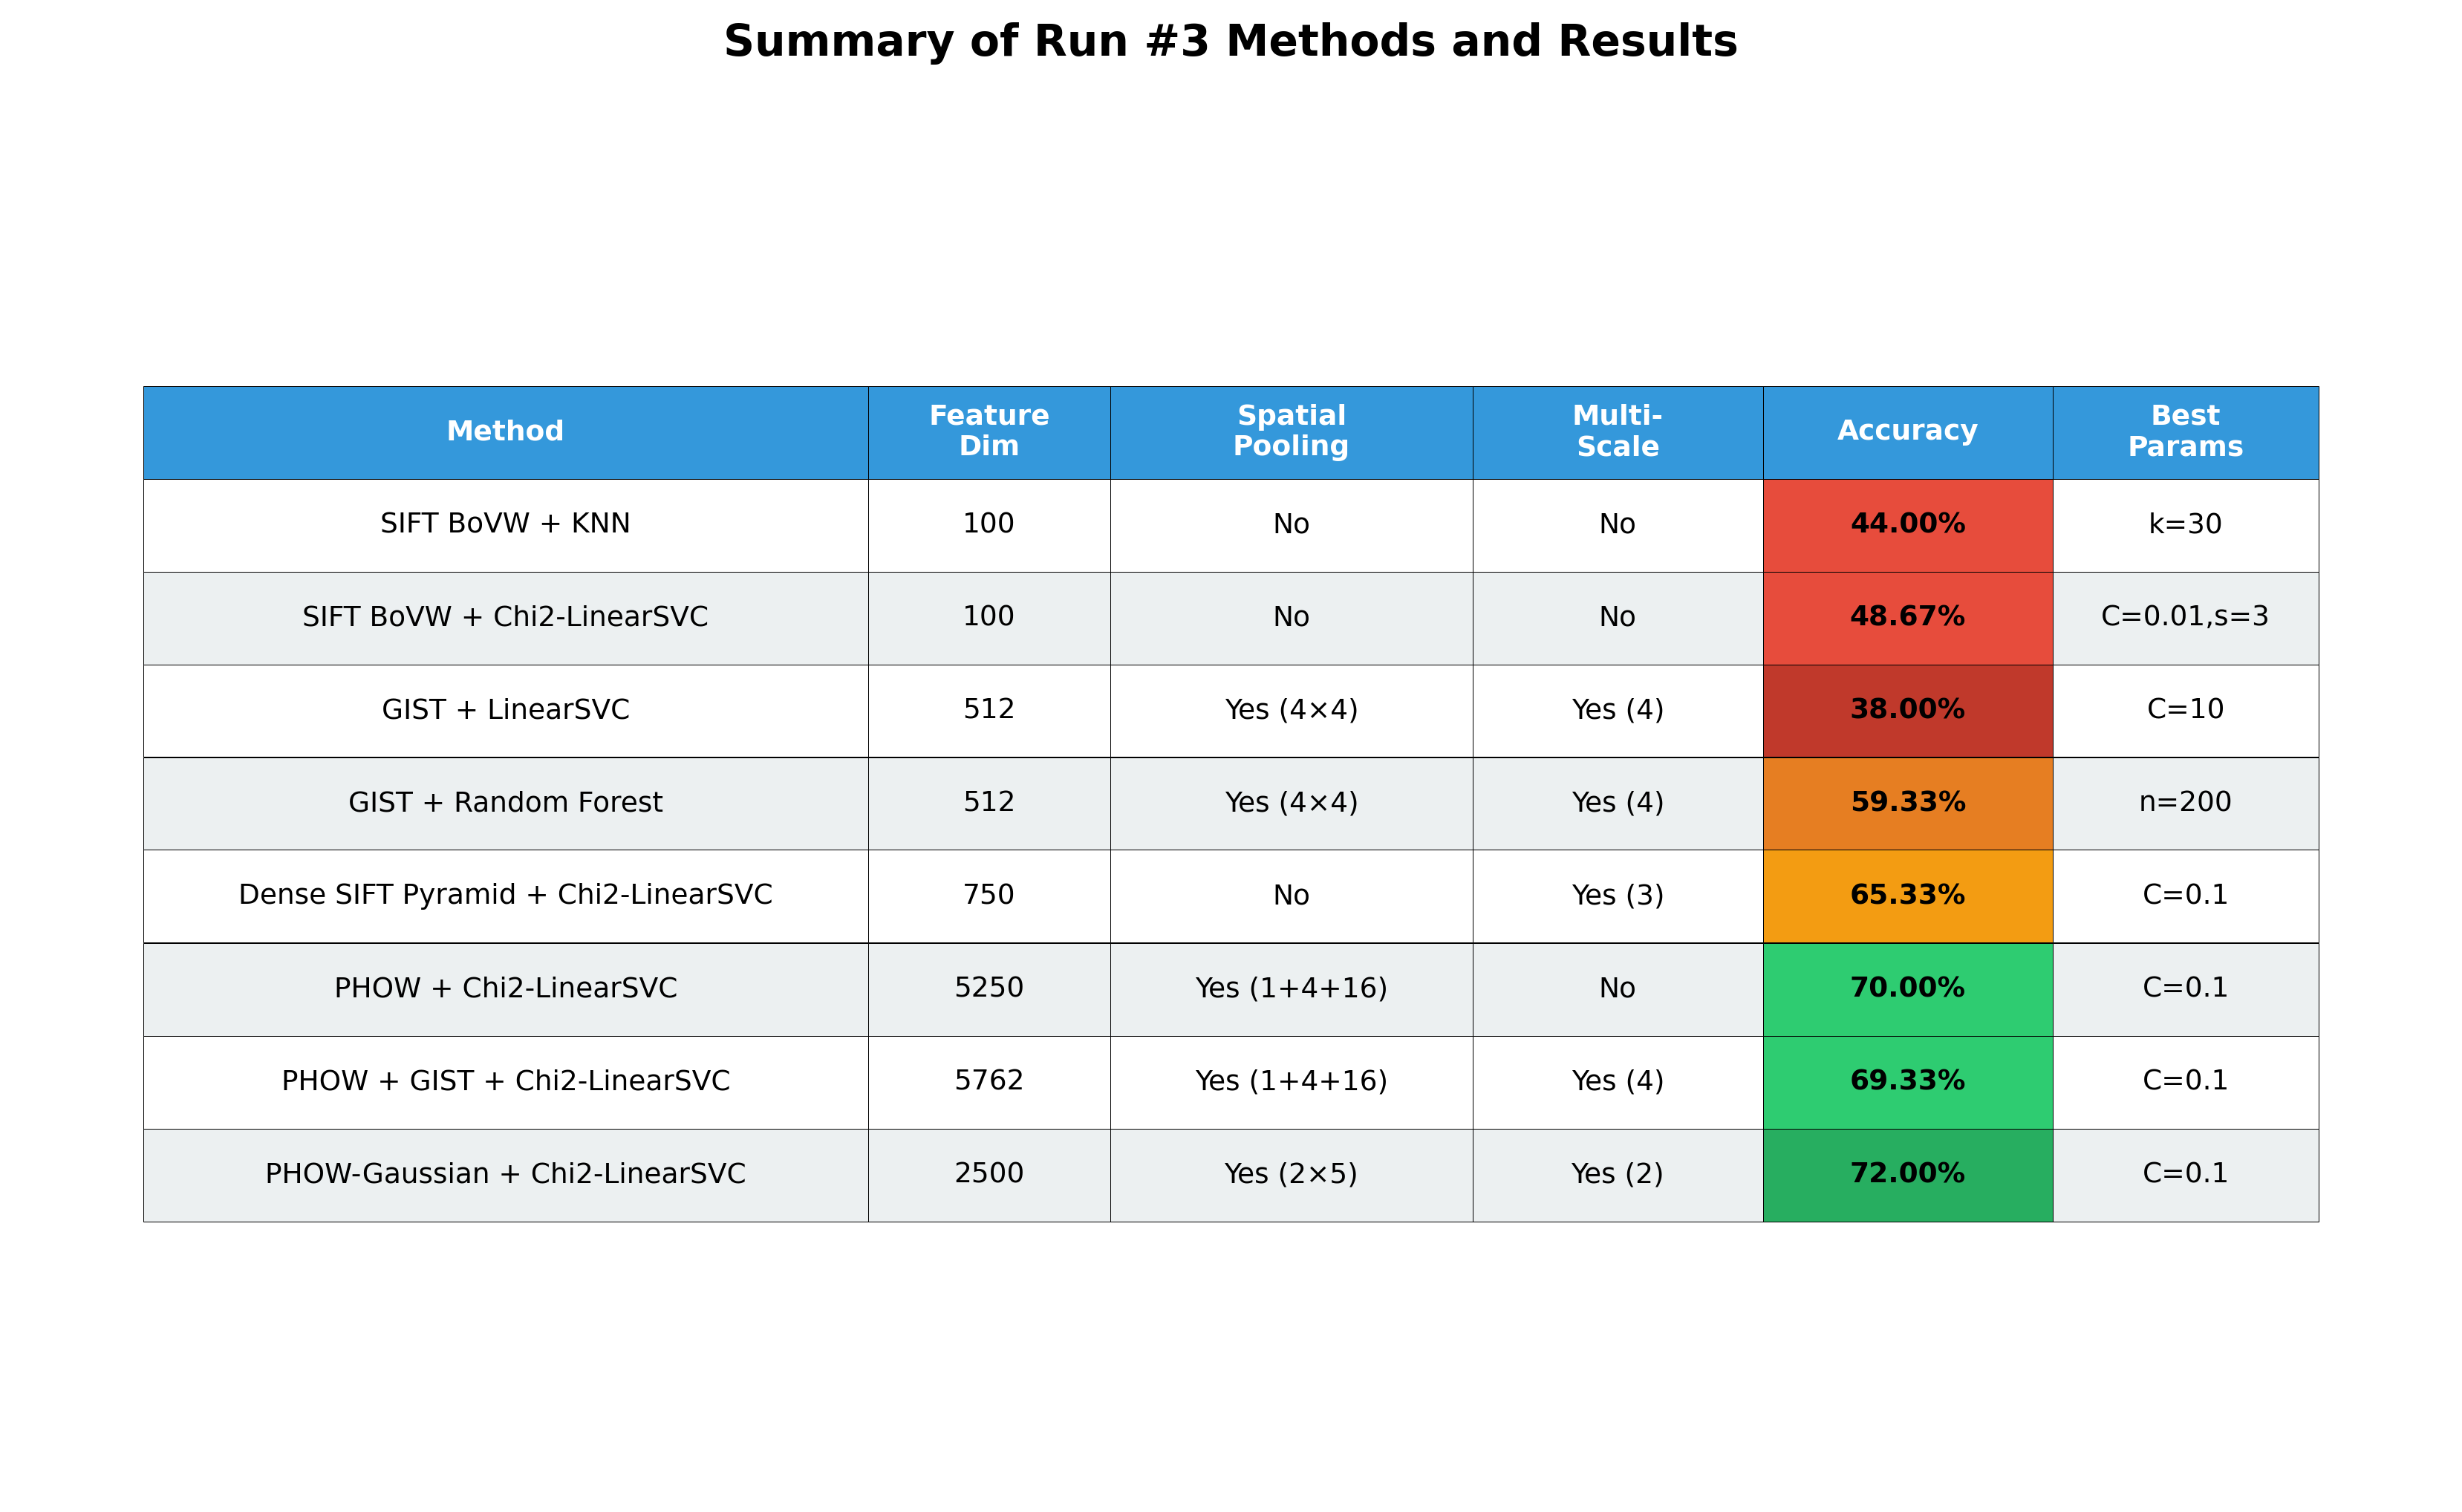
\includegraphics[width=\linewidth]{figures/fig7_summary_table.png}
\caption{Summary of all evaluated methods with best hyperparameter configurations and validation accuracies. Methods are ranked by performance, with PHOW-Gaussian+Chi2-SVM achieving the highest accuracy of 72.00\%. The table shows that spatial pyramid methods (PHOW-based) consistently outperform other approaches, and the optimal regularization parameter C varies significantly across feature types, with GIST requiring C=10 while pyramid methods work best with C=0.1.}
\label{tab:run3_results}
\end{figure}

Figure~\ref{tab:run3_results} summarizes the validation accuracy and optimal hyperparameter configurations for all evaluated methods. The results are ranked by accuracy, with PHOW-Gaussian Pyramid achieving 72.00\%, followed by PHOW (70.00\%) and PHOW+GIST fusion (69.33\%). Dense SIFT Pyramid reaches 65.33\%. Basic SIFT BoVW methods achieve 48.67\% with Chi2-LinearSVC (C=0.01, sample\_steps=3) and 44.00\% with k-NN (k=30). GIST with Random Forest achieves 59.33\%, substantially better than GIST with Linear SVM (38.00\%), highlighting the importance of classifier selection for different feature types.

Several key observations emerge from these experimental results. First, spatial information is more important than multi-scale information for scene recognition. PHOW (spatial pyramid only) achieves 70.00\%, while Dense SIFT Pyramid (Gaussian pyramid only) achieves 65.33\%, demonstrating a 4.67 percentage point advantage for spatial layout encoding. This suggests that knowing where features appear in the image is more discriminative than capturing features at multiple scales for the scene recognition task.

Second, combining both types of pyramids yields the best performance. PHOW-Gaussian reaches 72.00\%, which is 2\% higher than PHOW alone. This improvement indicates that multi-scale information does provide additional discriminative power when combined with spatial layout, even though it is less effective in isolation. The combination allows the model to capture both the spatial arrangement of scene elements and their scale variations.

Third, the choice of classifier significantly affects performance for different feature types. GIST benefits more from Random Forest (59.33\%) than Linear SVM (38.00\%), showing a 21.33 percentage point difference. This large gap suggests that GIST features have non-linear decision boundaries that Random Forest can model effectively, while Linear SVM cannot. In contrast, spatial pyramid features work well with Linear SVM when combined with Chi-Square kernel approximation, likely because the histogram-based representations are already in a suitable feature space.

Fourth, feature dimensionality alone does not determine performance. GIST uses only 512 dimensions but achieves moderate accuracy (59.33\%) with appropriate classifiers. PHOW-Gaussian uses 2500 dimensions and achieves the best accuracy, offering a good balance between performance and computational cost. PHOW uses 5250 dimensions but only achieves 70.00\%, demonstrating that very high dimensionality does not guarantee better results and may even lead to overfitting or increased computational burden without corresponding accuracy gains.

For the final Run 3 submission, we select PHOW-Gaussian Pyramid with Chi-Square kernel and Linear SVM (C=0.1) based on its validation accuracy of 72.00\%. The model is retrained on all 1500 training images and applied to the test set to generate predictions. This method represents the best combination of multi-scale feature extraction, spatial layout encoding, and appropriate classification strategy among all evaluated approaches.
%%%\end{comment}

%%%%%%%%% BODY TEXT
\section{Introduction}

Please follow the steps outlined below when submitting your manuscript to
the IEEE Computer Society Press.  This style guide now has several
important modifications (for example, you are no longer warned against the
use of sticky tape to attach your artwork to the paper), so all authors
should read this new version.

%-------------------------------------------------------------------------
\subsection{Language}

All manuscripts must be in English.

\subsection{Dual submission}

Please refer to the author guidelines on the CVPR 2020 web page for a
discussion of the policy on dual submissions.

\subsection{Paper length}
Papers, excluding the references section,
must be no longer than eight pages in length. The references section
will not be included in the page count, and there is no limit on the
length of the references section. For example, a paper of eight pages
with two pages of references would have a total length of 10 pages.
{\bf There will be no extra page charges for CVPR 2020.}

Overlength papers will simply not be reviewed.  This includes papers
where the margins and formatting are deemed to have been significantly
altered from those laid down by this style guide.  Note that this
\LaTeX\ guide already sets figure captions and references in a smaller font.
The reason such papers will not be reviewed is that there is no provision for
supervised revisions of manuscripts.  The reviewing process cannot determine
the suitability of the paper for presentation in eight pages if it is
reviewed in eleven.  

%-------------------------------------------------------------------------
\subsection{The ruler}
The \LaTeX\ style defines a printed ruler which should be present in the
version submitted for review.  The ruler is provided in order that
reviewers may comment on particular lines in the paper without
circumlocution.  If you are preparing a document using a non-\LaTeX\
document preparation system, please arrange for an equivalent ruler to
appear on the final output pages.  The presence or absence of the ruler
should not change the appearance of any other content on the page.  The
camera ready copy should not contain a ruler. (\LaTeX\ users may uncomment
the \verb'\cvprfinalcopy' command in the document preamble.)  Reviewers:
note that the ruler measurements do not align well with lines in the paper
--- this turns out to be very difficult to do well when the paper contains
many figures and equations, and, when done, looks ugly.  Just use fractional
references (e.g.\ this line is $095.5$), although in most cases one would
expect that the approximate location will be adequate.

\subsection{Mathematics}

Please number all of your sections and displayed equations.  It is
important for readers to be able to refer to any particular equation.  Just
because you didn't refer to it in the text doesn't mean some future reader
might not need to refer to it.  It is cumbersome to have to use
circumlocutions like ``the equation second from the top of page 3 column
1''.  (Note that the ruler will not be present in the final copy, so is not
an alternative to equation numbers).  All authors will benefit from reading
Mermin's description of how to write mathematics:
\url{http://www.pamitc.org/documents/mermin.pdf}.


\subsection{Blind review}

Many authors misunderstand the concept of anonymizing for blind
review.  Blind review does not mean that one must remove
citations to one's own work---in fact it is often impossible to
review a paper unless the previous citations are known and
available.

Blind review means that you do not use the words ``my'' or ``our''
when citing previous work.  That is all.  (But see below for
techreports.)

Saying ``this builds on the work of Lucy Smith [1]'' does not say
that you are Lucy Smith; it says that you are building on her
work.  If you are Smith and Jones, do not say ``as we show in
[7]'', say ``as Smith and Jones show in [7]'' and at the end of the
paper, include reference 7 as you would any other cited work.

An example of a bad paper just asking to be rejected:
\begin{quote}
\begin{center}
    An analysis of the frobnicatable foo filter.
\end{center}

   In this paper we present a performance analysis of our
   previous paper [1], and show it to be inferior to all
   previously known methods.  Why the previous paper was
   accepted without this analysis is beyond me.

   [1] Removed for blind review
\end{quote}


An example of an acceptable paper:

\begin{quote}
\begin{center}
     An analysis of the frobnicatable foo filter.
\end{center}

   In this paper we present a performance analysis of the
   paper of Smith \etal [1], and show it to be inferior to
   all previously known methods.  Why the previous paper
   was accepted without this analysis is beyond me.

   [1] Smith, L and Jones, C. ``The frobnicatable foo
   filter, a fundamental contribution to human knowledge''.
   Nature 381(12), 1-213.
\end{quote}

If you are making a submission to another conference at the same time,
which covers similar or overlapping material, you may need to refer to that
submission in order to explain the differences, just as you would if you
had previously published related work.  In such cases, include the
anonymized parallel submission~\cite{Authors14} as additional material and
cite it as
\begin{quote}
[1] Authors. ``The frobnicatable foo filter'', F\&G 2014 Submission ID 324,
Supplied as additional material {\tt fg324.pdf}.
\end{quote}

Finally, you may feel you need to tell the reader that more details can be
found elsewhere, and refer them to a technical report.  For conference
submissions, the paper must stand on its own, and not {\em require} the
reviewer to go to a techreport for further details.  Thus, you may say in
the body of the paper ``further details may be found
in~\cite{Authors14b}''.  Then submit the techreport as additional material.
Again, you may not assume the reviewers will read this material.

Sometimes your paper is about a problem which you tested using a tool which
is widely known to be restricted to a single institution.  For example,
let's say it's 1969, you have solved a key problem on the Apollo lander,
and you believe that the CVPR70 audience would like to hear about your
solution.  The work is a development of your celebrated 1968 paper entitled
``Zero-g frobnication: How being the only people in the world with access to
the Apollo lander source code makes us a wow at parties'', by Zeus \etal.

You can handle this paper like any other.  Don't write ``We show how to
improve our previous work [Anonymous, 1968].  This time we tested the
algorithm on a lunar lander [name of lander removed for blind review]''.
That would be silly, and would immediately identify the authors. Instead
write the following:
\begin{quotation}
\noindent
   We describe a system for zero-g frobnication.  This
   system is new because it handles the following cases:
   A, B.  Previous systems [Zeus et al. 1968] didn't
   handle case B properly.  Ours handles it by including
   a foo term in the bar integral.

   ...

   The proposed system was integrated with the Apollo
   lunar lander, and went all the way to the moon, don't
   you know.  It displayed the following behaviours
   which show how well we solved cases A and B: ...
\end{quotation}
As you can see, the above text follows standard scientific convention,
reads better than the first version, and does not explicitly name you as
the authors.  A reviewer might think it likely that the new paper was
written by Zeus \etal, but cannot make any decision based on that guess.
He or she would have to be sure that no other authors could have been
contracted to solve problem B.
\medskip

\noindent
FAQ\medskip\\
{\bf Q:} Are acknowledgements OK?\\
{\bf A:} No.  Leave them for the final copy.\medskip\\
{\bf Q:} How do I cite my results reported in open challenges?
{\bf A:} To conform with the double blind review policy, you can report results of other challenge participants together with your results in your paper. For your results, however, you should not identify yourself and should not mention your participation in the challenge. Instead present your results referring to the method proposed in your paper and draw conclusions based on the experimental comparison to other results.\medskip\\



\begin{figure}[t]
\begin{center}
\fbox{\rule{0pt}{2in} \rule{0.9\linewidth}{0pt}}
   %\includegraphics[width=0.8\linewidth]{egfigure.eps}
\end{center}
   \caption{Example of caption.  It is set in Roman so that mathematics
   (always set in Roman: $B \sin A = A \sin B$) may be included without an
   ugly clash.}
\label{fig:long}
\label{fig:onecol}
\end{figure}

\subsection{Miscellaneous}

\noindent
Compare the following:\\
\begin{tabular}{ll}
 \verb'$conf_a$' &  $conf_a$ \\
 \verb'$\mathit{conf}_a$' & $\mathit{conf}_a$
\end{tabular}\\
See The \TeX book, p165.

The space after \eg, meaning ``for example'', should not be a
sentence-ending space. So \eg is correct, {\em e.g.} is not.  The provided
\verb'\eg' macro takes care of this.

When citing a multi-author paper, you may save space by using ``et alia'',
shortened to ``\etal'' (not ``{\em et.\ al.}'' as ``{\em et}'' is a complete word.)
However, use it only when there are three or more authors.  Thus, the
following is correct: ``
   Frobnication has been trendy lately.
   It was introduced by Alpher~\cite{Alpher02}, and subsequently developed by
   Alpher and Fotheringham-Smythe~\cite{Alpher03}, and Alpher \etal~\cite{Alpher04}.''

This is incorrect: ``... subsequently developed by Alpher \etal~\cite{Alpher03} ...''
because reference~\cite{Alpher03} has just two authors.  If you use the
\verb'\etal' macro provided, then you need not worry about double periods
when used at the end of a sentence as in Alpher \etal.

For this citation style, keep multiple citations in numerical (not
chronological) order, so prefer \cite{Alpher03,Alpher02,Authors14} to
\cite{Alpher02,Alpher03,Authors14}.


\begin{figure*}
\begin{center}
\fbox{\rule{0pt}{2in} \rule{.9\linewidth}{0pt}}
\end{center}
   \caption{Example of a short caption, which should be centered.}
\label{fig:short}
\end{figure*}

%------------------------------------------------------------------------
\section{Formatting your paper}

All text must be in a two-column format. The total allowable width of the
text area is $6\frac78$ inches (17.5 cm) wide by $8\frac78$ inches (22.54
cm) high. Columns are to be $3\frac14$ inches (8.25 cm) wide, with a
$\frac{5}{16}$ inch (0.8 cm) space between them. The main title (on the
first page) should begin 1.0 inch (2.54 cm) from the top edge of the
page. The second and following pages should begin 1.0 inch (2.54 cm) from
the top edge. On all pages, the bottom margin should be 1-1/8 inches (2.86
cm) from the bottom edge of the page for $8.5 \times 11$-inch paper; for A4
paper, approximately 1-5/8 inches (4.13 cm) from the bottom edge of the
page.

%-------------------------------------------------------------------------
\subsection{Margins and page numbering}

All printed material, including text, illustrations, and charts, must be kept
within a print area 6-7/8 inches (17.5 cm) wide by 8-7/8 inches (22.54 cm)
high.
Page numbers should be in footer with page numbers, centered and .75
inches from the bottom of the page and make it start at the correct page
number rather than the 4321 in the example.  To do this fine the line (around
line 23)
\begin{verbatim}
%\ifcvprfinal\pagestyle{empty}\fi
\setcounter{page}{4321}
\end{verbatim}
where the number 4321 is your assigned starting page.

Make sure the first page is numbered by commenting out the first page being
empty on line 46
\begin{verbatim}
%\thispagestyle{empty}
\end{verbatim}


%-------------------------------------------------------------------------
\subsection{Type-style and fonts}

Wherever Times is specified, Times Roman may also be used. If neither is
available on your word processor, please use the font closest in
appearance to Times to which you have access.

MAIN TITLE. Center the title 1-3/8 inches (3.49 cm) from the top edge of
the first page. The title should be in Times 14-point, boldface type.
Capitalize the first letter of nouns, pronouns, verbs, adjectives, and
adverbs; do not capitalize articles, coordinate conjunctions, or
prepositions (unless the title begins with such a word). Leave two blank
lines after the title.

AUTHOR NAME(s) and AFFILIATION(s) are to be centered beneath the title
and printed in Times 12-point, non-boldface type. This information is to
be followed by two blank lines.

The ABSTRACT and MAIN TEXT are to be in a two-column format.

MAIN TEXT. Type main text in 10-point Times, single-spaced. Do NOT use
double-spacing. All paragraphs should be indented 1 pica (approx. 1/6
inch or 0.422 cm). Make sure your text is fully justified---that is,
flush left and flush right. Please do not place any additional blank
lines between paragraphs.

Figure and table captions should be 9-point Roman type as in
Figures~\ref{fig:onecol} and~\ref{fig:short}.  Short captions should be centred.

\noindent Callouts should be 9-point Helvetica, non-boldface type.
Initially capitalize only the first word of section titles and first-,
second-, and third-order headings.

FIRST-ORDER HEADINGS. (For example, {\large \bf 1. Introduction})
should be Times 12-point boldface, initially capitalized, flush left,
with one blank line before, and one blank line after.

SECOND-ORDER HEADINGS. (For example, { \bf 1.1. Database elements})
should be Times 11-point boldface, initially capitalized, flush left,
with one blank line before, and one after. If you require a third-order
heading (we discourage it), use 10-point Times, boldface, initially
capitalized, flush left, preceded by one blank line, followed by a period
and your text on the same line.

%-------------------------------------------------------------------------
\subsection{Footnotes}

Please use footnotes\footnote {This is what a footnote looks like.  It
often distracts the reader from the main flow of the argument.} sparingly.
Indeed, try to avoid footnotes altogether and include necessary peripheral
observations in
the text (within parentheses, if you prefer, as in this sentence).  If you
wish to use a footnote, place it at the bottom of the column on the page on
which it is referenced. Use Times 8-point type, single-spaced.


%-------------------------------------------------------------------------
\subsection{References}

List and number all bibliographical references in 9-point Times,
single-spaced, at the end of your paper. When referenced in the text,
enclose the citation number in square brackets, for
example~\cite{Authors14}.  Where appropriate, include the name(s) of
editors of referenced books.

\begin{table}
\begin{center}
\begin{tabular}{|l|c|}
\hline
Method & Frobnability \\
\hline\hline
Theirs & Frumpy \\
Yours & Frobbly \\
Ours & Makes one's heart Frob\\
\hline
\end{tabular}
\end{center}
\caption{Results.   Ours is better.}
\end{table}

%-------------------------------------------------------------------------
\subsection{Illustrations, graphs, and photographs}

All graphics should be centered.  Please ensure that any point you wish to
make is resolvable in a printed copy of the paper.  Resize fonts in figures
to match the font in the body text, and choose line widths which render
effectively in print.  Many readers (and reviewers), even of an electronic
copy, will choose to print your paper in order to read it.  You cannot
insist that they do otherwise, and therefore must not assume that they can
zoom in to see tiny details on a graphic.

When placing figures in \LaTeX, it's almost always best to use
\verb+\includegraphics+, and to specify the  figure width as a multiple of
the line width as in the example below
{\small\begin{verbatim}
   \usepackage[dvips]{graphicx} ...
   \includegraphics[width=0.8\linewidth]
                   {myfile.eps}
\end{verbatim}
}


%-------------------------------------------------------------------------
\subsection{Color}

Please refer to the author guidelines on the CVPR 2020 web page for a discussion
of the use of color in your document.

%------------------------------------------------------------------------
\section{Final copy}

You must include your signed IEEE copyright release form when you submit
your finished paper. We MUST have this form before your paper can be
published in the proceedings.

Please direct any questions to the production editor in charge of these 
proceedings at the IEEE Computer Society Press: 
\url{https://www.computer.org/about/contact}. 


{\small
\bibliographystyle{ieee_fullname}
\bibliography{egbib}
}


\end{document}
